\section{Human Activity Recognition}
\label{sec:soa:har}

%Talk about human activity recognition as a research topic. Explain in what application it has been used, how and for what and different sensor approaches used. Make clear that this dissertation will be based on sensor-based activity recognition.

Human activity recognition has become a key research topic in diverse areas, including pervasive and mobile computing \cite{Weiser1991} \cite{Choudhury2008}, surveillance-based security \cite{Poppe2010}, \cite{Akdemir2008}, \cite{Weinland2011}, context-aware computing \cite{Laerhoven2001}, \cite{Wren2006}, ambient assisted living \cite{Philipose2004}, \cite{Cook2009}, \cite{Kasteren2008}, \cite{Chen2012a} and social robotics \cite{Fong2003a}. The recent increase in interest in activity recognition can be attributed to the intensive thrusts from the latest technology development and application demands. The progress in sensor technologies has been substantial over the past decade, especially low-power, low-cost, high-capacity and miniaturised sensors, wired and wireless communication networks \cite{Pantelopoulos2010}, \cite{Alemdar2010}, \cite{Ding2011}. In parallel, data processing techniques have also shown important advances, based on higher computational capabilities of devices and the development of novel algorithms. The progress and maturity of these supporting technologies have pushed the research focuses of the aforementioned areas to shift from low-level data collection and transmission towards high-level information integration, context processing and activity recognition and inference. 

At the same time, activity recognition has been demanded by a growing number of solutions for real-world problems and applications. For example, surveillance and security try to make use of activity recognition technologies to address the threats of terrorists \cite{Akdemir2008}. Ambient assisted living aims to exploit activity monitoring, recognition and assistance to support independent living and ageing in place. Other emerging applications, such as intelligent meeting rooms \cite{Mikic2000} and smart hospitals \cite{Sanchez2008}, are also dependent on activity recognition in order to provide multimodal interactions, proactive service provision, and context aware personalised activity assistance. 

As a result of the technology push and application pull, activity recognition has built its own space in the academic world. As such, research related to activity recognition has become regular topics in mainstream international conferences in related areas such as the AAAI Conference on Artificial Intelligence\footnote{http://www.aaai.org/}, Computer Vision and Pattern Recognition\footnote{http://www.cvpr201x.org/}, International Joint Conference on Artificial Intelligence\footnote{http://ijcai.org/}, International Joint Conference on Pervasive and Ubiquitous Computing\footnote{http://ubicomp.org/}, International Conference on Pervasive Computing and Communications\footnote{http://www.percom.org/} and International Joint Conferences on Ambient Intelligence\footnote{http://www.ami-conferences.org/}. In order to try to channel the research towards future applications, a substantial number of projects and initiatives have been undertaken. Good examples are \textit{The Ambient Assisted Living Joint Programme}\footnote{www.aal-europe.eu}, \textit{The House of the Future}\footnote{http://architecture.mit.edu/house\_n}, \textit{The Gator-Tech Smart House}\footnote{http://www.icta.ufl.edu/gt.htm} or \textit{The iDorm project}\footnote{http://cswww.essex.ac.uk/iieg/idorm.htm}.  %In addition, a growing number of workshops have been dedicated to activity recognition research from different research angles and communities. For example, in 2011 alone eight workshops were specifically devoted to activity recognition research, including IWFAR [24], HAU3D [25], SAGAware [26], PAIR [27], GAPRec [28] and others [29][30][31]. The interest and enthusiasm for this topic is still increasing.

Apart from potential applications, activity recognition has gained research interest because it is a multidisciplinary and complex process. Activity recognition can be roughly characterised by four basic tasks. These tasks include:
\begin{enumerate}
 \item Selection and deployment of appropriate sensors to objects and environments in order to monitor and capture a user’s behaviour along with the state change of the environment.
 \item To collect, store and process perceived information through data analysis techniques and/or knowledge representation formalisms at appropriate levels of abstraction.
 \item To create computational activity models in a way that allows software systems/agents to conduct reasoning and manipulation.
 \item To select or develop reasoning algorithms to infer activities from sensor data.
\end{enumerate}

Each individual task can be tackled by a great variety of methods, technologies and tools. It is often the case that the selection of a method used for one task is dependent on the method of another task. As such, activity recognition has been classified in the following ways according to \cite{Chen2012}. The first classification criterion focuses on the sensors used for activity monitoring, while the second one pays attention to activity modelling techniques:

\begin{enumerate}
 \item \textit{Vision-based vs. sensor-based activity recognition:} In terms of the type of sensor that is used for activity monitoring, activity recognition can be generally classified into two categories. The first is referred to as vision-based activity recognition, which is based on the use of visual sensing facilities such as video cameras to monitor an actor’s behaviour and environmental changes. The generated sensor data are video sequences or digitized visual data. The approaches in this category exploit computer vision techniques, including feature extraction, structural modelling, person and object recognition, movement segmentation, action extraction and movement tracking to analyse visual observations for pattern recognition. The second category is referred to as sensor-based activity recognition, which is based on the use of emerging sensor network technologies for activity monitoring (Section \ref{sec:soa:sensor}). The generated sensor data from sensor-based monitoring are mainly time series of state changes and/or various parameter values that are usually processed through data fusion, probabilistic or statistical analysis methods and formal knowledge technologies for activity recognition. Sensor-based activity monitoring can be further classified into two categories: (i) wearable sensor-based activity monitoring, where sensors are attached to an actor under observation, and (ii) dense sensing-based activity monitoring, where sensors are attached to objects that constitute the activity environment. Wearable sensors, including modern smartphones, often use inertial measurement units and RFID tags to gather an actor’s behavioural information. This approach is effective for recognising physical movements such as physical exercises. In contrast, dense sensing infers activities by monitoring human-object interactions through the usage of multiple multi-modal miniaturised sensors.

 \item \textit{Data-driven vs. knowledge-driven activity recognition:} The information obtained through activity monitoring has to be structured and processed to recognise activities. For that purpose, activity models play a critical role. In particular, the mechanisms activities are recognised are closely related to the nature and representation of activity models. Generally speaking, activity models can be built using one of two methods. The first is to learn activity models from pre-existent large-scale datasets of users’ behaviours using data mining and machine learning techniques. This method involves the creation of probabilistic or statistical activity models, followed by training and learning processes. As this method is driven by data, and the ensued activity inference is based on probabilistic or statistical classification, it is often referred to as data-driven or bottom-up approaches (in the rest of this dissertation, data-driven will be used to refer to this category). The advantages of the data-driven approaches are the capabilities of handling uncertainty and temporal information \cite{Brand1997}. However, this method requires large datasets for training and learning, and suffers from the data scarcity or the “cold start” problem. It is also difficult to apply learnt activity models from one person to another. As such this method suffers from the problems of scalability and reusability. Data-driven approaches are described in detail in Section \ref{sec:soa:datadriven}. The other method for building activity models is to exploit rich prior knowledge in the domain of interest to construct activity models directly using knowledge engineering and management technologies. This usually involves knowledge acquisition, formal modelling and representation. Activity models generated in this method are normally used for activity recognition or prediction through formal logical reasoning, e.g., deduction, induction or abduction. As such, this method is referred to as knowledge-driven or top-down approach (knowledge-driven will be used from now on). Knowledge-driven approaches have the advantages of being semantically clear, logically elegant and easy to get started. But they are weak in handling uncertainty and temporal information and the models could be viewed as static and incomplete. For a complete review of knowledge-driven approaches, see Section \ref{sec:soa:knowledgedriven}. With the purpose of combining the advantages of those two methods, hybrid approaches have recently emerged (Section \ref{sec:soa:hybrid}). 
\end{enumerate}

The situation generated by both classification criteria is represented in Figure \ref{fig-classification}, providing a high-level view of activity recognition systems' taxonomy.

\begin{figure}[htbp]
\centering
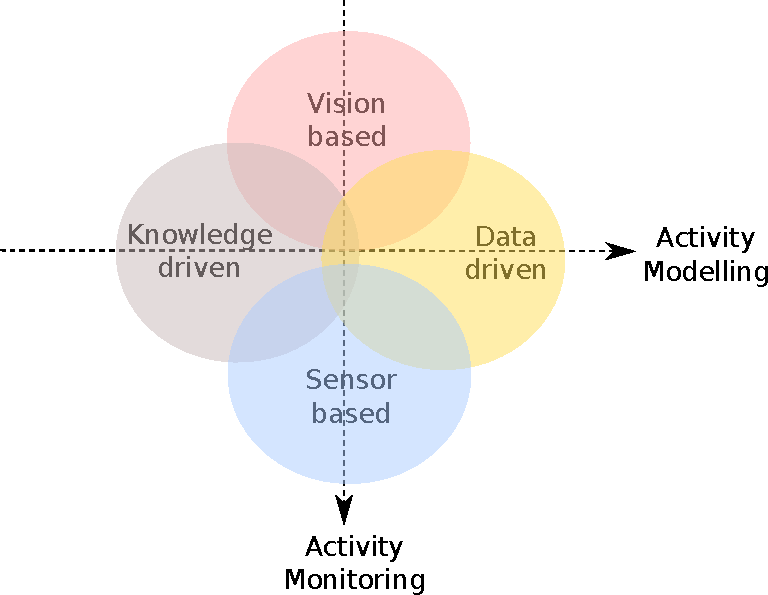
\includegraphics[width=11cm]{activity_taxonomy-m.pdf}
    \caption{A high-level taxonomy of activity recognition systems, spanned by two axis: monitoring and modelling approach.}
    \label{fig-classification}
\end{figure}
 
Vision-based activity recognition has been a research focus for a long period of time due to its important role in areas such as surveillance, robot learning and security. However, as this dissertation is based on sensor-based approaches, an exhaustive review of vision-based systems is not provided. Detailed up to date reviews can be found in \cite{Poppe2010}, \cite{Moeslund2006}, \cite{Yilmaz2006}, \cite{Weinland2011} and \cite{Turaga2008}. Even though all those surveys cover different topics, together they have provided an extensive overview on the vision-based approach. It is concluded from those contributions that while visual monitoring is intuitive and information-rich, vision-based activity recognition suffers from issues relating to privacy and ethics \cite{Yilmaz2006} as cameras are generally perceived as recording devices.

Compared to the number of surveys in vision-based activity recognition, and considering the wealth of literature in sensor-based activity recognition, there is a lack of extensive review on the state of the art of sensor-based activity recognition. This may be because the approach only recently became feasible when the sensing technologies matured to be realistically deployable in terms of the underpinning communication infrastructure, costs and sizes. An exception to this rule is the survey published by Chen et al. \cite{Chen2012}, which can be considered as the reference work for any sensor-based activity recognition approach. 

\section{Sensor-Based Activity Recognition}
\label{sec:soa:sensor}

For the upcoming discussions about activity monitoring, modelling and recognition, it is useful to distinguish human behaviours at different levels of granularity. For physical behaviours, the terms “action” and “activity” are commonly used in activity recognition communities. In some cases they are used interchangeably and in other cases they are used to denote behaviours of different complexity and duration. In the latter cases the term “action” is usually referred to as simple ambulatory behaviour executed by a single person and typically lasting for short durations of time. Examples of actions include bending, retrieving a cup from a cupboard, opening a door, putting a teabag into a cup and so forth. On the other hand, the term “activities” here refers to complex behaviours consisting of a sequence of actions and/or interleaving or overlapping actions. They could be performed by a single human or several humans who are required to interact with each other in a constrained manner. They are typically characterized by much longer temporal durations, such as making tea or two persons making meals. For the rest of this dissertation, the second case will be adopted. As such, ``actions'' will be considered short-time simple executions, while ``activities'' will be described by a sequence of actions.

The first approaches that implemented the idea of using sensors for activity monitoring and recognition appeared in the late 90s. The \textit{Neural Network House} \cite{Mozer1998}, in the context of home automation, can be considered a pioneer in this area, alongside with a number of location-based applications aiming to adapt systems to users’ whereabouts \cite{Leonhardt1998}, \cite{Golding1999}, \cite{Ward1997}. The approach was soon found to be more useful and suitable in the area of ubiquitous and mobile computing – an emerging area in the late 90s, due to its easy deployment. As such, extensive research has been undertaken to investigate the use of sensors in various application scenarios of ubiquitous and mobile computing, leading to considerable work on context-awareness \cite{Schmidt1999}, \cite{Randell2000}, \cite{Gellersen2002}, smart appliances \cite{Schmidt2001}, \cite{Laerhoven2001} and activity recognition \cite{Laerhoven2001a}, \cite{Foerster2000}, \cite{Lee2002}. Those initial research works usually made use of wearable sensors, either dedicated sensors attached to human bodies or portable devices like mobile phones, with application to ubiquitous computing scenarios such as providing context-aware mobile devices. Activities being monitored in these researches are mainly physical activities like motion, walking and running. These early works lay a solid foundation for wearable computing and still inspire and influence today’s research.

In the early 2000s, a new sensor-based approach that uses sensors attached to objects to monitor human activities appeared. This approach, which was later dubbed as the “dense sensing” approach, performs activity recognition through the inference of user-object interactions \cite{Bao2004}, \cite{Patterson2003}. The approach is particularly suitable for dealing with activities that involve a number of objects within an environment, or instrumental Activities of Daily Living (ADL) \cite{Chan2008}, \cite{Nugent2009}. Research on this approach has been heavily driven by the intensive research interests and huge research effort on smart home based assisted living, such as the EU’s Ambient Assisted Living program. In particular, sensor-based activity recognition can better address sensitive issues in assisted living such as privacy, ethics and obtrusiveness than conventional vision-based approaches. This combination of application needs and technological advantages has stimulated considerable research activities in a global scale, which gave rise to a large number of research projects, where a plethora of impressive works on sensor-based activity recognition have been developed \cite{Kern2003}, \cite{Mantyjarvi2001}, \cite{Philipose2004}, \cite{Patterson2005}, \cite{Buettner2009}, \cite{Wren2006}, \cite{Gu2009}, \cite{Patterson2003}, \cite{Liao2007}.

While substantial research has been undertaken, and significant progress has been made, the two main approaches, wearable sensors based and dense sensing based activity recognition are currently still focuses of study. The former is mainly driven by the ever-popular pervasive and mobile computing while the latter is predominantly driven by smart environment applications such as ambient assisted living. Interests in various novel applications are still increasing and application domains are rapidly expanding.

\section{Sensor and Activity Monitoring}
\label{sec:soa:monitoring}

Thanks to the rapid development in electronics, a wide range of sensors, including contact sensors, RFID, accelerometers, audio and motion detectors, to name but a few, are available for activity monitoring. These sensors are different in types, purposes, output signals, underpinning theoretical principles and technical infrastructure. However, they can be classified into two main categories in terms of the way they are deployed in activity monitoring applications. These are wearable sensors and dense sensors, and are described in detail in the following sections.

\subsection{Wearable sensor-based activity monitoring}

Wearable sensors generally refer to sensors that are positioned directly or indirectly on human body. These kinds of sensors can be worn by humans, so they are named wearable sensors. They generate signals when the user performs actions and activities. As a result, they can monitor features that are descriptive of the person’s physiological state or movement. Wearable sensors can be embedded into clothes, eyeglasses, belts, shoes, wristwatches, mobile devices or positioned directly on the body. They can be used to collect information such as body position and movement, pulse, and skin temperature. Researchers have found that different types of sensor information are effective for classifying different types of activities. As wearable sensors are not directly related to this dissertation, some references are shown for further reading, classified by the sensors used:

\begin{enumerate}
 \item Inertial measurement units: those sensors are composed by accelerometers and gyroscopes and are probably the most frequently used wearable sensor for activity monitoring. Inertial measurement units provide information about acceleration and speed of the units while moving. In consequence, they are appropriate to monitor human movements and actions and activities related to body motion, such as physical exercise. Some  examples of the usage of inertial measurement units are provided in \cite{Bao2004}, \cite{Lukowicz2004}, \cite{Lee2002} and \cite{Mantyjarvi2001}.
 \item GPS sensors: specially used for monitoring outdoor location-based activities, such as in \cite{Patterson2003}, \cite{Ashbrook2003} and \cite{Liao2007a}.
 \item Biosensors: to monitor activities through vital signs, e.g. \cite{Sung2004}, \cite{Harms2008} and \cite{Finni2007}.
\end{enumerate}

Wearable sensor-based activity monitoring suffers from limitations. Most wearable sensors need to run continuously and be operated hands-free. This may have difficulties in real world application scenarios. Practical issues include the acceptability or willingness to use wearable sensors and the viability and ability to wear them. Technical issues include the size, ease of use, battery life and effectiveness of the approach in real-world scenarios. A way to overcome such problems is to make use of existing gadgets that have already been carried in a daily basis like smartphones as intelligent sensors for activity monitoring, recognition and assistance. This practice has been in place for a while \cite{Gellersen2002}, \cite{Schmidt2001} and is expected to gain large-scale uptake given the latest development and affordability of such palm-held electronic devices. Recently, a new and promising class of wearable sensors have appeared in the market, namely the Google Glasses\footnote{https://www.google.com/glass/start/} (see Figure \ref{fig-google-glass}). Those special glasses include a camera, a small eye-screen, headphones and a computing unit. It is expected that the irruption of such glasses will bring to market more similar options. The potential of these kinds of devices for activity monitoring and recognition is still to be explored. 

Obviously wearable sensors are not suitable for monitoring activities that involve complex physical motions and/or multiple interactions with the environment. In some cases, sensor observations from wearable sensors alone are not sufficient to differentiate activities involving simple physical movements (e.g., making tea and making coffee). As a result, dense sensing based activity monitoring has emerged, which is described below.

\begin{figure}[htbp]
\centering
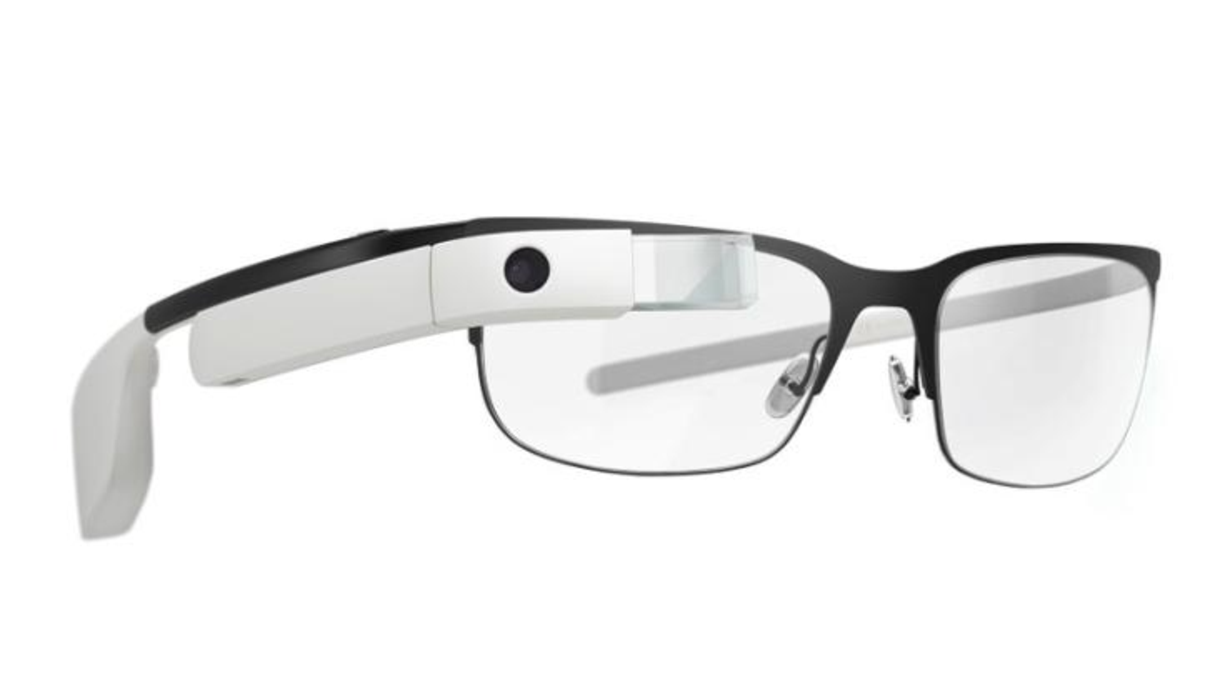
\includegraphics[width=9cm]{google-glass.pdf}
    \caption{The Google Glass wearable, with its processing unit, camera, headphones and screen.}
    \label{fig-google-glass}
\end{figure}

\subsection{Dense sensing-based activity monitoring}

Dense sensing-based activity monitoring is based on attaching sensors to objects that a user manipulates while performing activities. Hence activity monitoring is carried out by detecting user-object interactions. The approach is based on real-world observations that activities are characterised by the objects that are manipulated during their performance. A simple indication of an object being used can often provide powerful clues about the activity being undertaken. As such it is assumed that activities can be recognised from sensor data that monitors human interactions with objects in the environment. By dense sensing, the way and scale with which sensors are used is characterised. Using dense sensing a large number of sensors, normally low-cost low-power and miniaturised, are deployed in a range of objects or locations within an environment for the purpose of monitoring movement and behaviour. Following the dense sensing paradigm, sensors are moved from human bodies to human-populated environments.

The dense sensing paradigm has been widely used for creating ambient intelligent applications such as smart homes, because sensors are embedded within environments. The pre-eminence of dense sensing in ambient assisted living (AAL), via the smart home paradigm, can be seen in \cite{Chan2008}, \cite{Nugent2009} or \cite{Helal2005}. Sensors in a smart home can monitor an inhabitant’s movements and environmental events so that activities can be inferred based on the sensor observations, thus providing just-in-time context-aware assistance. For instance, a switch sensor in the bed can strongly suggest sleeping or relaxing, and pressure mat sensors can be used for tracking the movement and position of people within the environment.

Since the introduction of the idea in early 2000s \cite{Bao2004}, \cite{Patterson2003}, extensive research has been undertaken to investigate the applicability of the approach in terms of sensor types, modalities and applications. For example, Tapia et al. \cite{Tapia2004} use environmental state-change sensors to collect information about interaction with objects and recognise activities that are of interest to medical professionals such as toileting, bathing, and grooming. Wilson et al. \cite{Wilson2005} use four kinds of anonymous and binary sensors, motion detectors, break-beam sensors, pressure mats, and contact switches for simultaneous tracking and activity recognition. Wren et al. \cite{Wren2006} employ networks of passive infrared motion sensors to detect presence and movement of heat sources. With this captured data they can recognise low-level activities such as walking, loitering, and turning, as well as mid-level activities such as visiting and meeting. Srivastava et al. \cite{Srivastava2001} exploit wireless sensor network to develop smart learning environment for young children. Hollosi et al. \cite{Hollosi2010} use voice detection techniques to perform acoustic event classification for monitoring in Smart Homes. Simple object sensors are adopted in \cite{Aipperspach2006}.

Given the abundance of different types and modalities of sensors, sensors have been used in different ways and combinations for dense sensing activity monitoring in many application scenarios. It is impossible to claim that one sensor deployment for a specific application scenario is superior to the other. The suitability and performance is usually down to the nature of the type of activities being assessed and the characteristics of the concrete applications. 

Generally speaking, wearable sensor-based activity monitoring receives more attention in mobile computing while dense sensing is more suitable for intelligent environment enabled applications. It is worth pointing out that wearable sensors and dense sensing are not mutually exclusive. In some applications they have to work together. For example, RFID (Radio Frequency Identification) based activity monitoring requires that objects are instrumented with tags and users wear an RFID reader affixed to a glove or a bracelet. Philipose and Fishkin \cite{Philipose2004}, \cite{Fishkin2005} developed two devices, iGlove and iBracelet, working as wearable RFID readers that detect when users interact with unobtrusively tagged objects. Patterson et al. \cite{Patterson2005} performed fine-grained activity recognition (i.e., not just recognising that a person is cooking but determining what they are cooking) by aggregating abstract object usage. Hodges et al. \cite{Hodges2007} proposed to identify individuals from their behaviour based on their interaction with the objects they use in performing daily activities. Buettner et al. \cite{Buettner2009} recognise indoor daily activities by using an RFID sensor network. In most cases wearable sensors and dense sensing are complementary and can be used in combination in order to yield optimal recognition results. For example, Gu et al. \cite{Gu2009} combine wearable sensors and object sensors for collecting multimodal sensor information. Through a pattern-based method, they recognise sequential, interleaved and concurrent activities.

Dense sensing activity monitoring has also some drawbacks. One of the most obvious ones is the need to install a lot of sensors in human populated environments, which may involve considerable infrastructure changes (install pressure mats or movement sensors), or the problem of adding sensors to any new object introduced in the environment (attach contact sensors to glasses bought in the supermarket). The practical feasibility of the approach is probably linked to introducing sensors in the production steps of objects and building phases of the environments. Another drawback is the simple information provided by the sensors, which cannot be enough if very detailed activities have to be recognised. A contact sensor may indicate an interaction between a human and an object, but it cannot provide any information about how the object is being used by the human. 